\documentclass[10pt,a4paper,oneside]{99_fhnwreport}

%%%%%%%%%%%%%%%%%%%%%%%%%%%%%%%%%%%%%%%%%%%%%%%%%%%%%%%%%%%%%%%%%%%%%%%%%%%%%%%%
% basic font and language packages
%%%%%%%%%%%%%%%%%%%%%%%%%%%%%%%%%%%%%%%%%%%%%%%%%%%%%%%%%%%%%%%%%%%%%%%%%%%%%%%%
%\usepackage[left=20mm,right=20mm,top=20mm,bottom=20mm]{geometry}
\usepackage[T1]{fontenc} % font encoding
\usepackage{lmodern} % font latin modern
\usepackage[utf8]{inputenc} % input encoding
\usepackage[ngerman]{babel} % english and german word spelling
\usepackage[babel, german=swiss]{csquotes} % german cites
%\usepackage[babel, english=british]{csquotes} % english cites

%%%%%%%%%%%%%%%%%%%%%%%%%%%%%%%%%%%%%%%%%%%%%%%%%%%%%%%%%%%%%%%%%%%%%%%%%%%%%%%%
% style packages
%%%%%%%%%%%%%%%%%%%%%%%%%%%%%%%%%%%%%%%%%%%%%%%%%%%%%%%%%%%%%%%%%%%%%%%%%%%%%%%%
\usepackage{hyperref} % use hyperlinks in table of contents
\hypersetup{colorlinks=true,urlcolor=blue,linkcolor=black} % define hyperlink colors
\usepackage{verbatim} % don't interpret latex symbols (source code)
\usepackage{enumerate} % numbered items
\usepackage{graphicx} % use figures
\usepackage{subfigure} % more than one figure in the same place
\usepackage{booktabs} % create tables
\usepackage{multirow} % create tables
\usepackage{cite} % citations
\usepackage{pdflscape} % allow landscape sites in pdf documents
%\usepackage{pdfpages} % include pdf files

%%%%%%%%%%%%%%%%%%%%%%%%%%%%%%%%%%%%%%%%%%%%%%%%%%%%%%%%%%%%%%%%%%%%%%%%%%%%%%%%
% mathematical packages
%%%%%%%%%%%%%%%%%%%%%%%%%%%%%%%%%%%%%%%%%%%%%%%%%%%%%%%%%%%%%%%%%%%%%%%%%%%%%%%%
\usepackage{amsmath} % formula
\usepackage{amsfonts} % formula
\usepackage{amssymb} % formula
\usepackage{amsthm} % formula
\usepackage{listings} % source code formatting

%%%%%%%%%%%%%%%%%%%%%%%%%%%%%%%%%%%%%%%%%%%%%%%%%%%%%%%%%%%%%%%%%%%%%%%%%%%%%%%%
% optional parameters
%%%%%%%%%%%%%%%%%%%%%%%%%%%%%%%%%%%%%%%%%%%%%%%%%%%%%%%%%%%%%%%%%%%%%%%%%%%%%%%%
\bibliographystyle{IEEEtran}
\graphicspath{{./graphics}}

% source code parameters
\lstset{numbers=left, numberstyle=\tiny, numbersep=6pt}
\lstset{captionpos=b, tabsize=4, basicstyle=\small, xleftmargin=0mm, xrightmargin=0mm}

%%%%%%%%%%%%%%%%%%%%%%%%%%%%%%%%%%%%%%%%%%%%%%%%%%%%%%%%%%%%%%%%%%%%%%%%%%%%%%%%
% debugging parameters
%%%%%%%%%%%%%%%%%%%%%%%%%%%%%%%%%%%%%%%%%%%%%%%%%%%%%%%%%%%%%%%%%%%%%%%%%%%%%%%%
\usepackage{todonotes}
\overfullrule=1em

%%%%%%%%%%%%%%%%%%%%%%%%%%%%%%%%%%%%%%%%%%%%%%%%%%%%%%%%%%%%%%%%%%%%%%%%%%%%%%%%
% document settings
%%%%%%%%%%%%%%%%%%%%%%%%%%%%%%%%%%%%%%%%%%%%%%%%%%%%%%%%%%%%%%%%%%%%%%%%%%%%%%%%
%\title{Title\\\large Undertitle}
\title{
	\textsc{\LARGE{Pflichtenheft}}\\[10mm]
	\textsc{\LARGE{Mehrdimensionale Raumerfassung mittels Ultraschall}}
}

\author{}

\date{06.10.2016}

%%%%%%%%%%%%%%%%%%%%%%%%%%%%%%%%%%%%%%%%%%%%%%%%%%%%%%%%%%%%%%%%%%%%%%%%%%%%%%%
% pictures
%\begin{figure}[htb]
%\includegraphics[width=100mm]{image1.png}
%\figcaption{image1} % picture caption
%\label{fig:image1}
%\end{figure}
%
%(Abb. \ref{fig:image1})
%%%%%%%%%%%%%%%%%%%%%%%%%%%%%%%%%%%%%%%%%%%%%%%%%%%%%%%%%%%%%%%%%%%%%%%%%%%%%%%

%%%%%%%%%%%%%%%%%%%%%%%%%%%%%%%%%%%%%%%%%%%%%%%%%%%%%%%%%%%%%%%%%%%%%%%%%%%%%%%
% equation
%\begin{equation}
%X_{1,2} = \frac{-b \pm \sqrt{b^{2}-4ac}}{2a}
%\label{eq:equation1}
%\end{equation}
%%%%%%%%%%%%%%%%%%%%%%%%%%%%%%%%%%%%%%%%%%%%%%%%%%%%%%%%%%%%%%%%%%%%%%%%%%%%%%%

%%%%%%%%%%%%%%%%%%%%%%%%%%%%%%%%%%%%%%%%%%%%%%%%%%%%%%%%%%%%%%%%%%%%%%%%%%%%%%%
% table
%\begin{table}[tb]
%\centering
%\begin{tabular}
%
%\end{tabular}
%\caption{Table 1}
%\label{tab:table1}
%\end{table}
%%%%%%%%%%%%%%%%%%%%%%%%%%%%%%%%%%%%%%%%%%%%%%%%%%%%%%%%%%%%%%%%%%%%%%%%%%%%%%%

%%%%%%%%%%%%%%%%%%%%%%%%%%%%%%%%%%%%%%%%%%%%%%%%%%%%%%%%%%%%%%%%%%%%%%%%%%%%%%%
% citation
%\cite{BUCH1}
%%%%%%%%%%%%%%%%%%%%%%%%%%%%%%%%%%%%%%%%%%%%%%%%%%%%%%%%%%%%%%%%%%%%%%%%%%%%%%%

%%%%%%%%%%%%%%%%%%%%%%%%%%%%%%%%%%%%%%%%%%%%%%%%%%%%%%%%%%%%%%%%%%%%%%%%%%%%%%%
% source code
%\begin{lstlisting}[frame=tb,caption={Application.java}, label=lst:code, language=java]
%your source code
%\end{lstlisting}
% or
%\lstinputlisting[frame=tb,caption={Caption 1}, label=lst:code1, language=c]{path/file.src}
%
%%%%%%%%%%%%%%%%%%%%%%%%%%%%%%%%%%%%%%%%%%%%%%%%%%%%%%%%%%%%%%%%%%%%%%%%%%%%%%%

\begin{document}
%%%%%%%%%%%%%%%%%%%%%%%%%%%%%%%%%%%%%%%%%%%%%%%%%%%%%%%%%%%%%%%%%%%%%%%%%%%%%%%%
% title page
%%%%%%%%%%%%%%%%%%%%%%%%%%%%%%%%%%%%%%%%%%%%%%%%%%%%%%%%%%%%%%%%%%%%%%%%%%%%%%%%
\pagenumbering{gobble}
\maketitle

%\definecolor{gray}{rgb}{0.5,0.5,0.5}
%\color{gray}
\noindent % einzug
\rule{\linewidth}{0.5mm}

\textsc{
\begin{tabbing}
\hspace{40mm}	\= \hspace{15mm} \=\kill
Auftraggeber	\> FHNW, Hochschule für Technik \\[5mm]
Betreuung	\> Richard Gut, FHNW, Institut für Mikroelektronik \\
		\> Matthias Meier, FHNW, Institut für Automation \\[5mm]
Team		\> Raphael Mijnssen, \textup{raphael.mijnssen@students.fhnw.ch} \\
		\> Jonas Plüss, \textup{jonas.pluess@students.fhnw.ch} \\[5mm]
Studiengang	\> Elektro- und Informationstechnik \\[5mm]
\end{tabbing}
}

\rule{\linewidth}{0.5mm}
%\clearpage
\color{black}

%%%%%%%%%%%%%%%%%%%%%%%%%%%%%%%%%%%%%%%%%%%%%%%%%%%%%%%%%%%%%%%%%%%%%%%%%%%%%%%%
% table of contents
%%%%%%%%%%%%%%%%%%%%%%%%%%%%%%%%%%%%%%%%%%%%%%%%%%%%%%%%%%%%%%%%%%%%%%%%%%%%%%%%
\pagenumbering{roman}
\setcounter{page}{1}
\tableofcontents
\clearpage

%%%%%%%%%%%%%%%%%%%%%%%%%%%%%%%%%%%%%%%%%%%%%%%%%%%%%%%%%%%%%%%%%%%%%%%%%%%%%%%%
% Einleitung
%%%%%%%%%%%%%%%%%%%%%%%%%%%%%%%%%%%%%%%%%%%%%%%%%%%%%%%%%%%%%%%%%%%%%%%%%%%%%%%%
\pagenumbering{arabic}
\setcounter{page}{1}
\section{Ausgangslage}\label{sec:ausgangslage}
Nicht ohne Grund hat die Evolution die Fledermaus mit einem aussergewöhnlichen Sinn zur Orientierung im Raum ausgestattet. Die Möglichkeit, anhand der Echos von hochfrequenten akustischen Schallwellen Informationen über den Raum und mögliche Hindernissen zu gewinnen, ist eine spannende Alternative gegenüber dem rein optischen Sehsinn. So ist die Fledermaus z.B. nicht auf grosse Mengen Licht angewiesen. Auch aus der heutigen Medizinaltechnologie und der Zerstörungsfreien Materialprüfung (engl. non-destructive testing) ist Ultraschall nicht mehr wegzudenken. Die Möglichkeit mit relativ billigen Ressourcen Informationen über den Raum gewinnen zu können oder das Innere von Strukturen und Objekten zu untersuchen, ohne diese zu beschädigen wird dabei ausgenützt. Es werden dafür je nach Art und Position der zu untersuchenden Struktur unterschiedliche Reflektionen der Ultraschallwellen gemessen. Die zu diesem Zweck erzeugten Schallwellen werden in der Regel mittels piezoelektrischem Effekt erzeugt. Wenn anstelle eines einzelnen Senders ein ganzes Array von Sendern verwendet wird, kann die Richtwirkung des resultierenden Sendekegels verbessert werden, sowie mittels elektrischer Zeitverzögerungen (Phasenverschiebung) bei der Ansteuerung die Richtung des Kegels geändert werden.

Umsetzungen dieser Technologien sind teuer und die Produkte in der Regel kommerziell, daher finden sich kaum öffentlich zugängige Projekte.

Ziel ist die Umsetzung eines Ultraschall Phased Array Systems, welches eindimensional in Luft aufgebaut wird und mit welchem die Objekterkennung im Raum ermöglicht wird. Es soll dabei sowohl Hardware, als auch Software entwickelt werden, welche unter GPL/Creative-Commons Lizenz steht und möglichst simpel, bzw. preiswert realisiert ist.
Als Basis dient das vorausgehende Projekt, wobei mittels funktionierendem Prototyp die Machbarkeit geprüft wurde und theoretische Grundlagen erarbeitet wurden. Dieser Prototyp wird durch ein Hardware Redesign bezüglich der Kosten, der Nebenkeulenunterdrückung und der minimalen messbaren Distanz optimiert. Die Signalverarbeitung der empfangenen Daten wird in einer dafür geeigneten Programmiersprache umgesetzt und dem GUI übergeben, welches möglichst Plattformunabhängig sein sollte. Die Visualisierung der Daten und die Steuerung der Hardware erfolgen über das GUI.

\clearpage

%%%%%%%%%%%%%%%%%%%%%%%%%%%%%%%%%%%%%%%%%%%%%%%%%%%%%%%%%%%%%%%%%%%%%%%%%%%%%%%%
% Ziele
%%%%%%%%%%%%%%%%%%%%%%%%%%%%%%%%%%%%%%%%%%%%%%%%%%%%%%%%%%%%%%%%%%%%%%%%%%%%%%%%
\section{Ziele}\label{sec:ziele}
Das Ziel des Projektes ist es, ein 1x8 Ultraschall Phased Array System zu entwickeln, welches der Objekterkennung in Luft dient. Im vorhergehenden Projekt wurde ein Prototyp gebaut, mit welchem bereits die Machbarkeit eines solchen Systems untersucht wurde. Dieser Prototyp wird bezüglich Unterdrückung der Nebenkeulen, Kosten und Auflösung für kleine Distanzen optimiert und dafür einem Hardware Redesign unterzogen. Die Signalverarbeitung der empfangen Echos wird in Software auf einem Linux Rechner in einer dafür geeigneten Programmiersprache implementiert und die Daten mit einem plattformunabhängigen GUI visualisiert. Zusätzlich wird die Steuerung der Hardware auch über dieses GUI erfolgen.

\subsection*{Sollziele}
\begin{itemize}
	\item Maximale Messdistanz: $5-10 \mathrm{m}$
	\item Minimale Tiefenauflösung: $\pm 10 \mathrm{cm}$
	\item Verwenden des gleichen Piezoelementes beim Senden und Empfangen
	\item Verkürzung der Abklingzeit der Piezoelemente
	\item Redesign der Hardware
	\item Verbesserung der Richtwirkung durch Amplitudenbelegung
	\item Anpassung der Firmware an Hardware Redesign
	\item Anpassung der Firmware für eine Steuerung per GUI
	\item Evaluation der verwendeten Programmiersprachen/Schnittstellen
	\item Implementation der Signalverarbeitung in der evaluierten Programmiersprache
	\item Implementation der Visualisierung der Daten
	\item Erstellen eines GUI
	\item Messen der Richtcharakteristik im Schalltoten Raum (siehe Testkonzept)
	\item Messen der Performance (Objekterkennung) im freien Feld (siehe Testkonzept)
\end{itemize}

\subsection*{Wunschziele}
\begin{itemize}
	\item Externes Sendemodul für Positionsbestimmung entwickeln
	\item Anpassung der Firmware/Software für Zusammenarbeit mit externem Sendemodul
	\item Darstellung der Positonsdaten des externen Sendemoduls
\end{itemize}

\clearpage

%%%%%%%%%%%%%%%%%%%%%%%%%%%%%%%%%%%%%%%%%%%%%%%%%%%%%%%%%%%%%%%%%%%%%%%%%%%%%%%%
% Loesungskonzept
%%%%%%%%%%%%%%%%%%%%%%%%%%%%%%%%%%%%%%%%%%%%%%%%%%%%%%%%%%%%%%%%%%%%%%%%%%%%%%%%
\section{Lösungskonzept}\label{sec:loesungskonzept}
Im nachfolgenden Kapitel wird erläutert, wie die bestehenden Probleme in der Hardware gelöst werden sollen und wie die Weiterentwicklung der Software aussehen soll. Das Lösungskonzept für das in den Wunschzielen aufgeführte externe Sendemodul wird separat betrachtet. Die grundlegende Struktur des Systems ist in der Abbildung \ref{fig:image_schema} ersichtlich.

%%%%%%%%%%%%%%%%%%%%%%%%%%%%%%%%%%%%%%%%%%%%%%%%%%%%%%%%%%%%%%%%%%%%%%%%%%%%%%%
% pictures
\begin{figure}[htb]
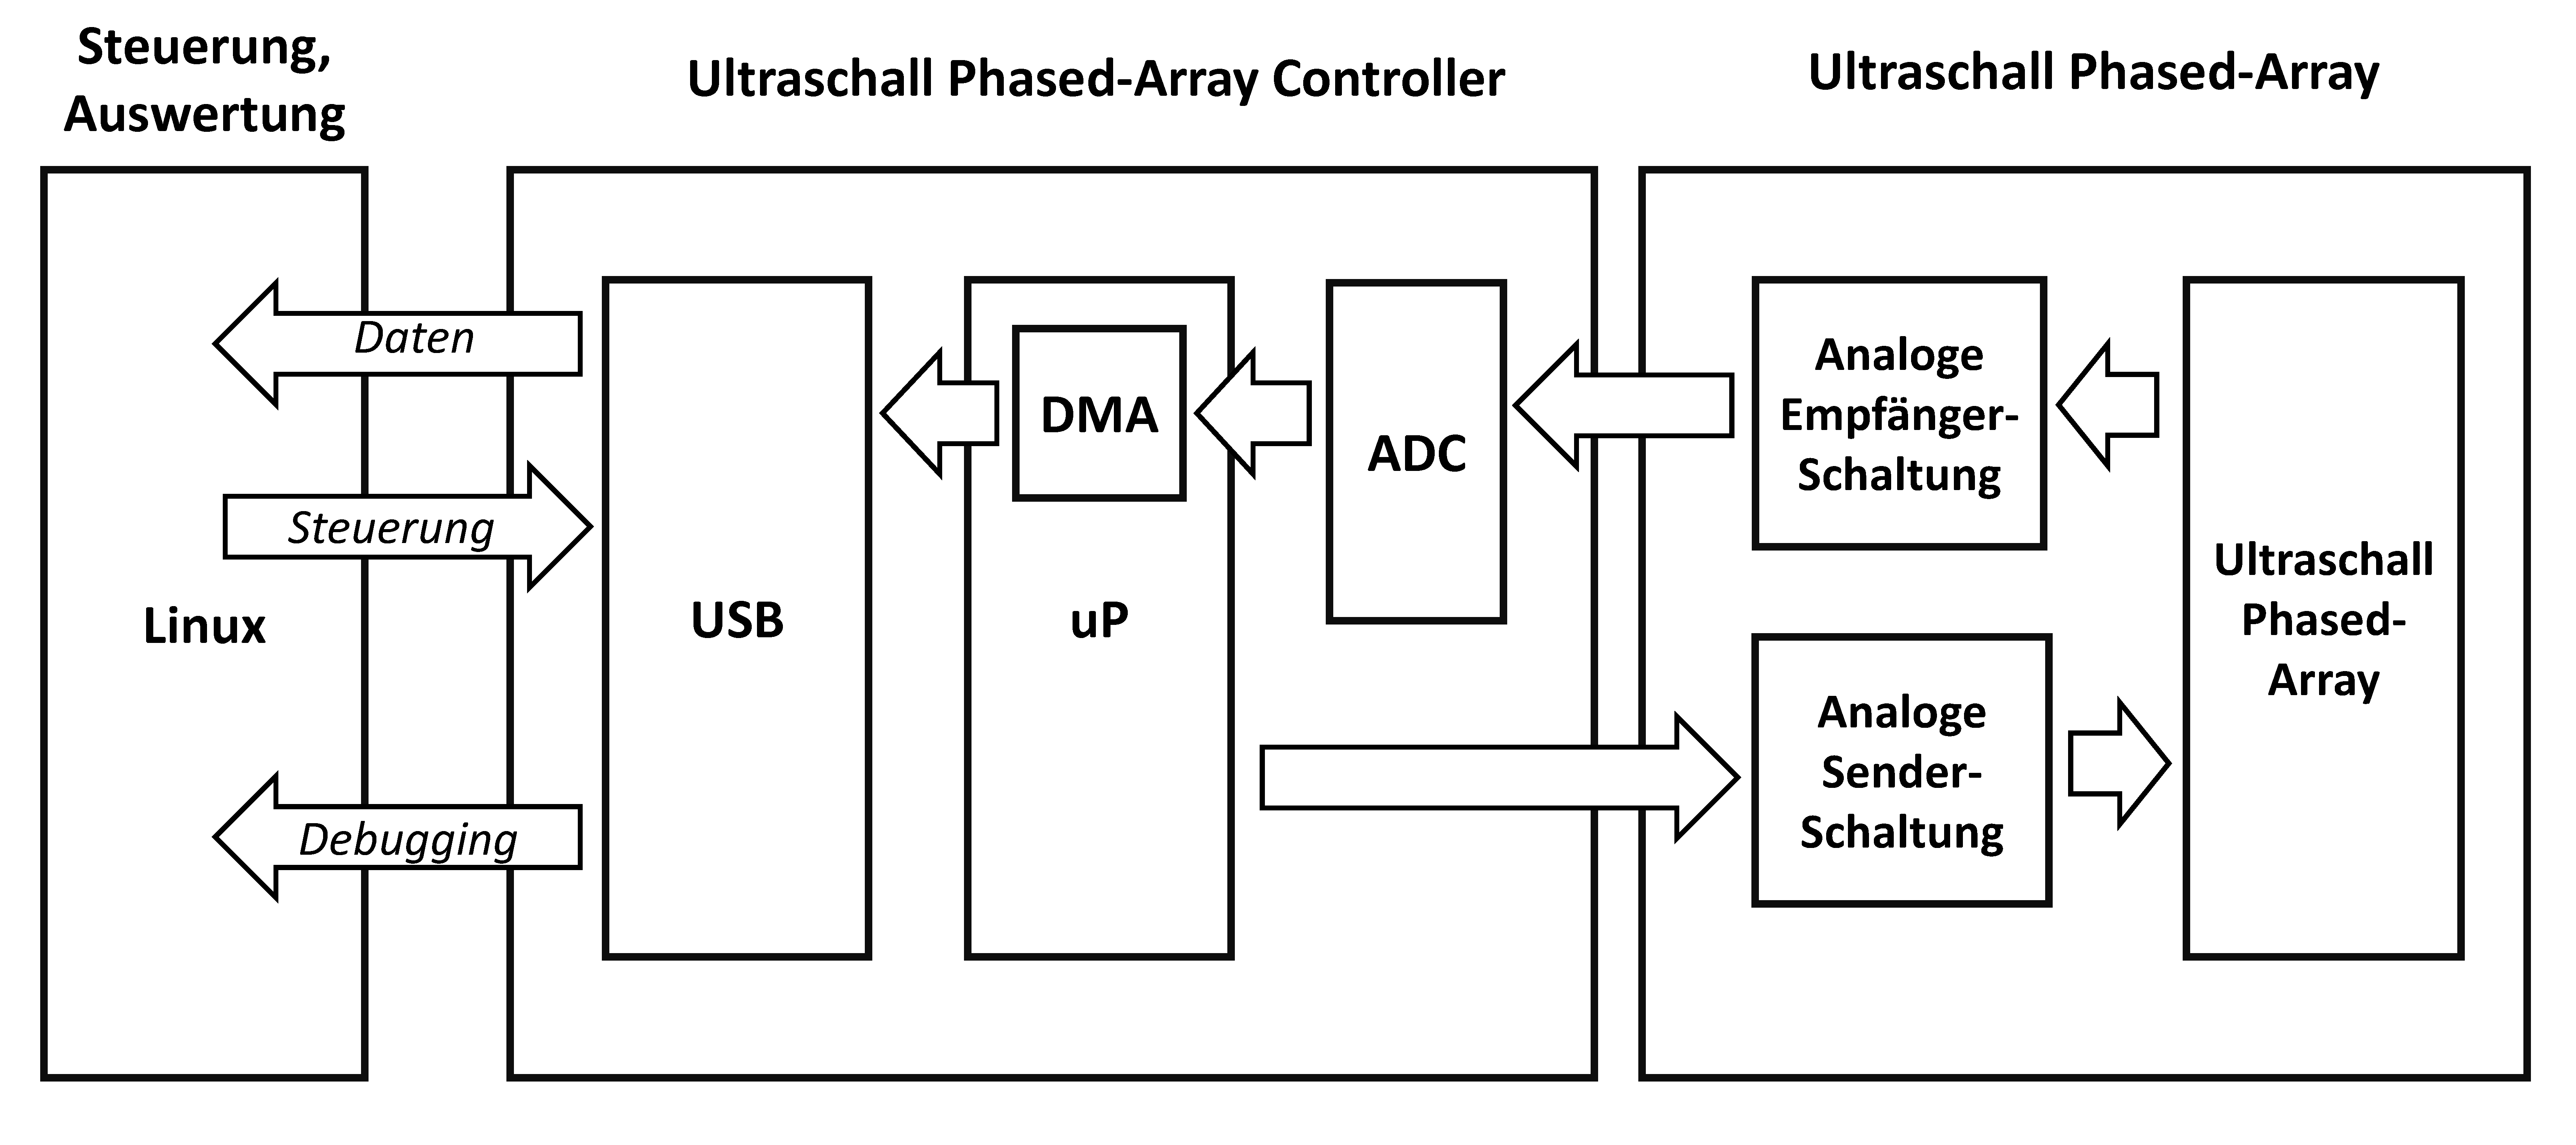
\includegraphics[width=\textwidth,angle=0]{graphics/image_schema.png}
\caption{Gesamtübersicht des Systems} % picture caption
\label{fig:image_schema}
\end{figure}
%
%(Abb. \ref{fig:image1})
%%%%%%%%%%%%%%%%%%%%%%%%%%%%%%%%%%%%%%%%%%%%%%%%%%%%%%%%%%%%%%%%%%%%%%%%%%%%%%%

%-------------------------------------------------------------------------------
\subsection*{Hardware}
Die im letzten Projekt entwickelte Hardware funktioniert zwar, weist aber einige kleine Schwächen auf, welche behoben werden sollen. Zwischen den Ultraschallsendern und -empfängern findet ein relativ starkes Übersprechen statt, was zusammen mit der langen Abklingzeit der Module dafür verantwortlich ist, dass jeweils zu Beginn des Empfangens noch keine Echos detektiert werden können. Diese zeitliche Verzögerung vergrössert die minimal erkennbare Distanz des Phased Arrays. In zwei Schritten soll dieser Umstand verbessert werden:

\begin{itemize}
	\item Aufbau mit nur einem Sender-/Empfängermodul, um Übersprechen zu verhindern.
	\item Verkürzung der Abklingzeit durch Dämpfen des Ausschwingens der Ultraschallmodule.
\end{itemize}

Um Gewissheit zu haben, dass die Verbesserungen auch funktionieren, werden die Konzepte zuerst auf einer Versuchsschaltung mit einem Ultraschallmodul aufgebaut und erst bei erfolgreichen Tests im Phased Array implementiert.

\subsubsection*{Versuche 1 \& 2 -- Evaluation für das Hardware Redesign}
Auf einer Versuchsplatine wird ein Schaltkreis mit nur einem Sender-/Empfängermodul aufgebaut. Dabei sind folgende Punkte wichtig:

\begin{itemize}
	\item Die beiden Vorspannungen an den Operationsverstärkern der Empfängerschaltung werden nicht über einzelne Spannungsteiler sondern über eine gemeinsame aktive Spannungsquelle erzeugt.
	\item Die Empfängerschaltung soll während dem Sendevorgang abkoppelbar sein.
	\item Über einen Steuerpin soll ein $1 \mathrm{k\Omega}$-Widerstand parallel zum Ultraschallmodul geschaltet werden können, um die Abklingzeit zu verkürzen.
\end{itemize}

Die Abkoppelung der Empfängerschaltung und das Zuschalten des Widerstandes soll mithilfe eines MOSFETs oder einer PIN-Diode geschehen. Die Vorspannung am Operationsverstärker wird mithilfe einer Spannungsfolgerschaltung (Impedanzwandler) mit einem weiteren Operationsverstärker erzeugt.

\subsubsection*{Redesign der Hardware}
Aufbauend auf den Erkenntnissen aus den Versuchen 1 \& 2 wird der Hardware Redesign gemacht. Für alle Vorspannungen an den Operationsverstärkern soll dieselbe aktive Spannungsquelle verwendet werden. Um schnelle Spannungsschwankungen zu verhindern, wird vor jedem Operationsverstärker ein Blockkondensator eingesetzt. Ansonsten wird die Beschaltung aus dem letzten Projekt übernommen. Das Umschalten der Ultraschallmodule zwischen Sender- und Empfängerschaltung soll für alle Module über einen einzelnen Pin gesteuert werden können, wie auch das Zuschalten des parallelen Widerstandes, falls sich dieser Ansatz gegen das Phasenverschobene Ansteuern (siehe Lösungskonzept Software) durchsetzt.

%-------------------------------------------------------------------------------
\subsection*{Software -- Firmware}
Verursacht durch das Hardware Redesign müssen auch an der Firmware einige Änderungen gemacht werden. Zusätzlich wird eine Softwareschnittstelle eingebaut, über die das Phased Array gesteuert werden kann.

\subsubsection*{Anpassung der Firmware an Hardware Redesign}
Um die Ultraschallmodule zwischen Sender- und Empfangsschaltung umzuschalten, sowie um die Widerstände zum Verkürzen der Abklingzeit dazuzuschalten müssen zusätzliche Pins per Software angesteuert werden.

Ein zweiter Ansatz zum Verkürzen der Abklingzeit ist das um $180 \mathrm{^{\circ}}$ Phasenverschobene Ansteuern der Sendemodule am Ende des Sendevorgangs. Es wird versucht, dies in der Firmware zu implementieren. Aufgrund des problematischen PWM-Timings im Atmel Software Framework (ASF) kann es aber sein, dass dieser Versuch scheitert. Dann bliebe nur noch das Dämpfen mithilfe eines parallel zum Sendemodul geschalteten Widerstandes.

\subsubsection*{Anpassung der Firmware für Amplitudenbelegung}
Um eine Nebenkeulenunterdrückung am Senderarray zu erreichen, kann die Amplitude der einzelnen Sendemodule mit einer Fensterfunktion belegt werden. Da die Anregung der Sendemodule mit einer PWM geschieht, kann die Pulsbreite entsprechend der gewünschten Sendeleistung angepasst werden.

\subsubsection*{Anpassung der Firmware für Steuerung über GUI}
Um das Ultraschall Phased Array über das GUI steuern zu können, muss die Firmware ebenfalls angepasst werden. Dazu wird wie auch zum Senden der Daten vom Phased Array zum PC die USB-Schnittstelle verwendet. Folgende Parameter sollen per GUI auf dem Phased Array Modul verändert werden können:

\begin{itemize}
	\item Sendewinkel
	\item Anzahl der Empfangsbuffer und somit die Empfangszeit
	\item Amplitudenbelegung
\end{itemize}

%-------------------------------------------------------------------------------
\subsection*{Software -- Signalverarbeitung / Visualisierung}
Die Software, welche die Daten des Phased Arrays auswertet, wird grob unterteilt in Signaverarbeitung und GUI. Eine erste rudimentäre Visualierung der Daten wird in Python geschrieben, um einen groben Überblick über die empfangen Daten zu erzielen.
Danach werden die optimalen Programmiersrachen und Schnittstellen für die Umsetzung evaluiert.

\subsubsection*{Signalverarbeitung}
Die Signalverarbeitung läuft auf einem Linuxrechner. Die Interpolation soll dabei nicht mittels Upsampling und Filterung im Zeitbereich, sondern im Bildbereich mithilfe der FFT realisiert werden. So kann Rechenzeit eingespart werden. Daraufhin soll die Enveloppe des Signals gebildet werden.  Diese wird danach zusammen mit dem Winkel dem GUI übergeben.

\subsubsection*{GUI}
Das GUI soll möglichst plattformunabhängig sein, evtl. Browserbasiert mit Javascript oder als Java Applet. Als Schnitstelle zwischen GUI und Signalvearbeitung kann womöglich TCP/IP oder Unix Sockets verwendet werden.
Die empfangenen Enveloppen werden jeweils für jeden Winkel aufgetragen. Dabei wird die Distanz (Zeit) als Strecke und die Signalamplitude als Farbe dargestellt.

%-------------------------------------------------------------------------------
\subsection*{Externes Sendemodul}
Optional soll ein externes Sendemodul aufgebaut werden, das vom Phased Array Modul angepingt werden kann und darauf aktiv ein kurzes Ultraschallsignal sendet. Das Phased Array empfängt dieses Signal und berechnet aus der Phasenverschiebung den Eintrittswinkel und aus der Signallaufzeit die Distanz zum externen Modul.

\subsubsection*{Pingsignal}
Damit die Signallaufzeit berechnet werden kann, muss das externe Sendemodul vom Phased Array getriggert werden. Dazu gibt es mehrere Lösungsansätze. Es könnte ein Ultraschallsignal, ein Funksignal oder ein Lichtsignal (Infrarot) verwendet werden. Beim triggern mittels Ultraschall entsteht einerseits die doppelte Signallaufzeit, andererseits könnten Reflexionen vom Phased Array falsch interpretiert werden. Die anderen beiden Lösungsansätze sind deshalb vorzuziehen.

\subsubsection*{Mikrocontroller}
Da nur ein Pingsignal empfangen und daraufhin ein Ultraschallsignal ausgesendet werden muss und keinerlei Signalverarbeitung auf dem externen Sendemodul stattfindet, werden an den Mikrocontroller keine hohen Anforderungen gestellt. Ein einfacher Atmega oder Attiny, welcher über einen Hardwareinterruptpin und einen PWM-Ausgang verfügt, sollte ausreichen. Für erste Tests wird dazu ein Arduino Nano verwendet.

\subsubsection*{Ultraschallmodul}
Da nur ein Sendemodul benötigt wird, kann dazu eigentlich jedes Ultraschallmodul mit $40 \mathrm{kHz}$ Resonanzfrequenz verwendet werden. Je höher dabei der Schalldruckpegel ist, desto weitere Distanzen können ausgemessen werden. Dabei ist aber darauf zu achten, dass die Empfänger des Phased Arrays nicht übersteuert werden.

\clearpage


%%%%%%%%%%%%%%%%%%%%%%%%%%%%%%%%%%%%%%%%%%%%%%%%%%%%%%%%%%%%%%%%%%%%%%%%%%%%%%%%
% Testkonzept
%%%%%%%%%%%%%%%%%%%%%%%%%%%%%%%%%%%%%%%%%%%%%%%%%%%%%%%%%%%%%%%%%%%%%%%%%%%%%%%%
\section{Testkonzept}\label{sec:testkonzept}
Im folgenden Kapitel wird das Testkonzept vorgestellt. Für eine zeitliche Übersicht sei dafür auf Abbildung \ref{fig:img_zeitplan} verwiesen.

%-------------------------------------------------------------------------------
\subsection*{Verifikation der Versuche 1 \& 2 -- Evaluation für das Hardware Redesign}
Es wird eine Testschaltung aufbaut, wobei nur ein Piezoelement für Sende- und Empfangsschaltung verwendet wird. Diese Schaltung wird mittels angepasster Firmware auf Funktionalität geprüft. Als zweiter Schritt wird die Dämpfung der Sensoren im Vergleich zum vorherigen Prototyp ohne Dämpfung verglichen. Es soll so festgestellt werden, wie klein der minimal messbare Abstand zum Sender ist. Dafür wird die Zeit gemessen, nach welcher die Amplitude des Signal am Ausgang der Verstärkerschaltung auf -26dB gedämpft ist im Vergleich zu den Aussteuerbaren 3.3 V.

%-------------------------------------------------------------------------------
\subsection*{Tests nach Redesign der Hardware}
Die fertiggestellte Hardware wird bezüglich Richtwirkung, Winkelauflösung und Distanz getestet. Dafür wird im schalltoten Raum der Schalldruck in Abhängigkeit des Winkels und der Distanz vermessen. Die Wirkung der Amplitdudenbelegung auf die Unterdrückung der Nebenkeulen wird dabei auch vermessen.

%-------------------------------------------------------------------------------
\subsection*{Tests nach fertigstellung der Software}
Nach der Fertigstellung der Software wird das Gesamtsystem getestet. Dafür werden Testobjekte zuerst im schalltoten Raum und danach im freien Feld vermessen. Die Resultate werden direkt im GUI dargestellt.
Falls das externe Sendemodul (optionales Ziel) entwickelt worden ist, wird für dieses die minimale Ortsauflösung und die maximal messbare Distanz ermittelt. Testmessungen sollen daraufhin im GUI dargestellt werden.

\clearpage


%%%%%%%%%%%%%%%%%%%%%%%%%%%%%%%%%%%%%%%%%%%%%%%%%%%%%%%%%%%%%%%%%%%%%%%%%%%%%%%%
% Projektplan
%%%%%%%%%%%%%%%%%%%%%%%%%%%%%%%%%%%%%%%%%%%%%%%%%%%%%%%%%%%%%%%%%%%%%%%%%%%%%%%%
%%%%%%%%%%%%%%%%%%%%%%%%%%%%%%%%%%%%%%%%%%%%%%%%%%%%%%%%%%%%%%%%%%%%%%%%%%%%%%%
% pictures
\begin{figure}[htb]
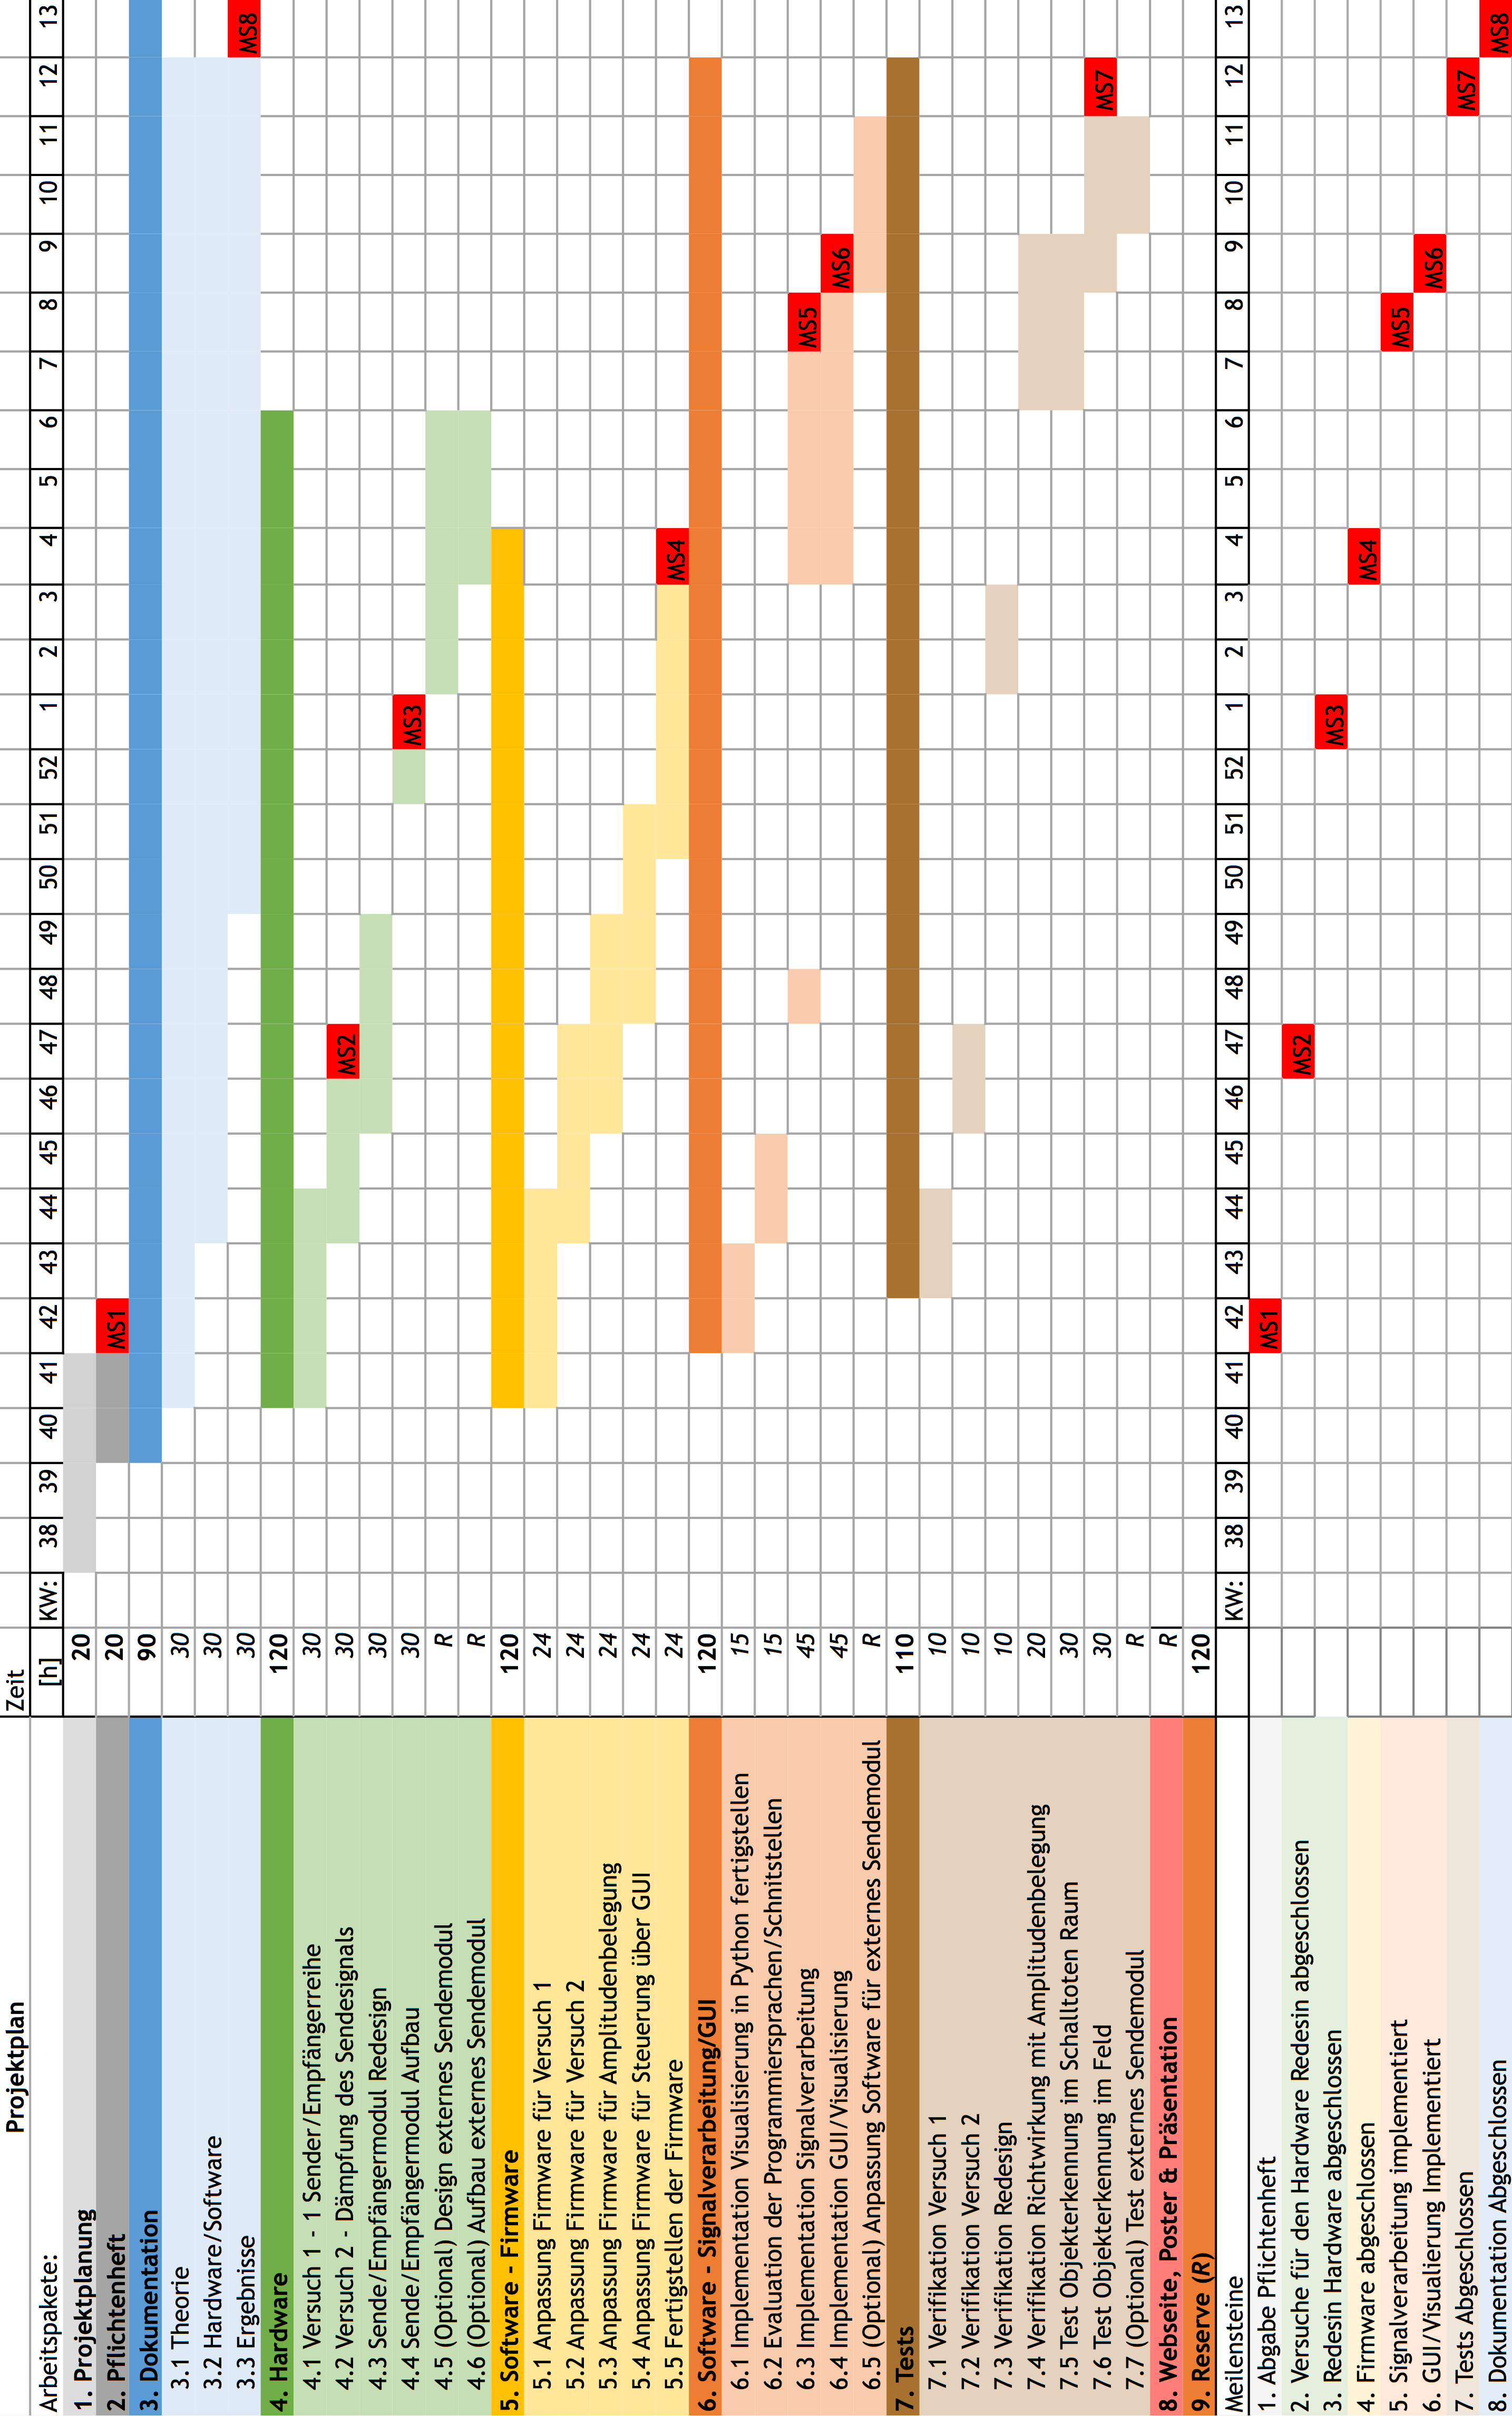
\includegraphics[width=0.9\textwidth,angle=0]{graphics/image_zeitplan.png}
\caption{Zeitplan \& Meilensteine} % picture caption
\label{fig:img_zeitplan}
\end{figure}
%
%(Abb. \ref{fig:image1})
%%%%%%%%%%%%%%%%%%%%%%%%%%%%%%%%%%%%%%%%%%%%%%%%%%%%%%%%%%%%%%%%%%%%%%%%%%%%%%%

\clearpage
\section{Projektplan}\label{sec:projektplan}
In diesem Kapitel wird das Zeitmanagement dieses Projektes behandelt. Der Projektplan gibt einen Überblick über die durchzuführenden Arbeiten, deren Zeitliche Einteilung und die Meilensteine welche zu erreichen sind. In einem Weiteren Abschnitt werden die einzelnen Arbeitspakete genauer beschrieben.


%%%%%%%%%%%%%%%%%%%%%%%%%%%%%%%%%%%%%%%%%%%%%%%%%%%%%%%%%%%%%%%%%%%%%%%%%%%%%%%%
% Arbeitspakete
%%%%%%%%%%%%%%%%%%%%%%%%%%%%%%%%%%%%%%%%%%%%%%%%%%%%%%%%%%%%%%%%%%%%%%%%%%%%%%%%
\subsection*{Arbeitspakete}\label{sec:arbeitspakete}
Im Folgenden werden die im Zeitplan (Abbildung \ref{fig:img_zeitplan}) aufgelisteten Arbeitspakete beschrieben.


%-------------------------------------------------------------------------------
\subsubsection*{1. Projektplanung}
Während der Projektplanung werden die Ergebnisse des letzten Projektes ausgewertet und das Lastenheft für das neue Projekt mit dem Auftraggeber besprochen. Die für dieses Projekt relevanten Dokumentvorlagen werden erstellt. Es wird ein Zeitplan ausgearbeitet, in welchem ersichtlich ist, wer zu welcher Zeit wieviele Stunden am Projekt arbeitet. Parallel dazu wird ein Zeitplan in Form eines Gantt-Diagrammes erstellt, in welchem alle Arbeitspakete, die Meilensteine sowie die dazu benötigte Zeit ersichtlich sind.


%-------------------------------------------------------------------------------
\subsubsection*{2. Pflichtenheft}
Das Pflichtenheft beschreibt konkret, was die Ziele dieses Projekts sind und wie sie umgesetzt werden. Es soll am Schluss des Projektes als Referenz zum Vergleich mit den Resultaten zur Verfügung stehen. Zusätzlich dient es der Orientierung und Planung während des Projektverlaufs. Die während der Projektplanung erstellten Zeitpläne sind Bestandteil des Pflichtenheftes.


%-------------------------------------------------------------------------------
\subsubsection*{3. Dokumentation}
Am Ende des Projektes wird ein Fachbericht abgegeben, welcher während der Projektdurchführung ausgearbeitet wird. Er beinhaltet die theoretischen Grundlagen der Akustik und der benötigten Signalverarbeitung sowie die Dokumentation der Hardware, der Software und der Ergebnisse. Das Ziel des Fachberichtes ist es, dass getroffene Entscheidungen nachvollzogen werden können, die Funktionsweise der Hard-/Software verständlich ist und die Tests reproduziert werden können.

\paragraph{3.1 Theorie}\\
Die theoretischen Grundlagen werden aufbauend auf dem im letzten Projekt erarbeiteten Wissen erweitert. Hauptsächlich wird der Teil der Signalverarbeitung verfeinert, sowie die Theorie zur Aperturbelegung bei Phased Array's zur Unterdrückung der Nebenkeulen erarbeitet.

\paragraph{3.2 Hardware / Software}\\
Aufbauend auf der Dokumentation aus dem letzten Projekt werden die Hardware und die Software im Top-Down Prinzip beschrieben. Für eine Fachperson soll es möglich sein, getroffene Entscheidungen nachzuvollziehen, die Hardware nachzubauen und die Software sowie die Entwicklungsumgebung in Betrieb zu nehmen.

\paragraph{3.3 Ergebnisse}\\
Die während dem Projekt gemachten Tests und Messungen werden in den Ergebnissen dokumentiert und sollen reproduzierbar sein.
In diesem Teil der Dokumentation werden ebenfalls Empfehlungen zur Weiterentwicklung des Projektes gemacht, welche aus zeitlichen Gründen nicht realisiert werden konnten.


%-------------------------------------------------------------------------------
\subsubsection*{4. Hardware}
Da zwischen den Ultraschallsendern und -empfängern ein relativ starkes Übersprechen stattfindet, welches die minimale Empfangsdistanz einschränkt, wird die Hardware einem Redesign unterzogen. Dabei können ev. auch noch zusätzliche Funktionalitäten eingebaut werden.

\paragraph{4.1 Versuch 1 -- Sender/Empfängerreihe}\\
Als erstes wird ein Aufbau getestet, bei dem zum Senden und zum Empfangen dasselbe Ultraschallmodul verwendet wird. Dies verhindert ein Übersprechen zwischen den Sende- und Empfangsmodulen und spart Kosten. Dazu wird kein ganzes Array aufgebaut, sondern nur ein einzelnes Modul getestet.

\paragraph{4.2 Versuch 2 -- Dämpfung des Sendesignals}\\
Wenn das Ultraschallmodul nach dem Senden um $180 \mathrm{^{\circ}}$ Phasenverschoben angesteuert wird, sollte es relativ schnell gedämpft werden können. Sollte dies aufgrund des Mikrocontrollers nicht möglich sein, wird nach dem Senden für kurze Zeit ein Widerstand parallel zum Sendemodul geschaltet, welcher dieses dämpft.

\paragraph{4.3 Sende-/Empfängermodul Redesign}\\
Den Ergebnissen der Versuche 1 und 2 entsprechend wird die komplette Hardware einem Redesign unterzogen, wobei die in den Versuchen getesteten Verbesserungen implementiert werden.

\paragraph{4.4 Sende-/Empfängermodul Aufbau}\\
Nach der Anfertigung des PCB werden die Komponenten darauf verbaut. Es sollen mindestens zwei, besser drei Module aufgebaut werden.

\paragraph{4.5 (Optional) Design externes Sendemodul}\\
Eine zusätzliche Möglichkeit des Phased Arrays auf dem Empfängermodul ist die zweidimensionale Ortung einer externen Ultraschallquelle. Mithilfe von zwei Empfängermodulen (eines horizontal und eines vertikal angeordnet) könnte sogar eine dreidimensionale Ortung stattfinden. In diesem Arbeitspaket soll ein externes Sendemodul entwickelt werden, welches vom Sende-/Empfängermodul angepingt werden kann und danach ein Signal aussendet welches vom Empfängerarray aufgenommen wird.

\paragraph{4.6 (Optional) Aufbau externes Sendemodul}\\
Nach dem Entwickeln des externen Sendemoduls wird es aufgebaut und getestet.

%-------------------------------------------------------------------------------
\subsubsection*{5. Software -- Firmware}
Das Redesign der Hardware erfordert auch einige Änderungen an der Firmware auf dem Mikrocontroller. Diese wird schrittweise immer dann angepasst, wenn die entsprechenden Änderungen an der Hardware erfolgreich abgeschlossen wurden.

\paragraph{5.1 Anpassung der Firmware für Versuch 1}\\
Die Firmware muss so angepasst werden, dass sie die Ultraschallmodule im richtigen Moment zwischen der Sendeelektronik und der Empfängerelektronik hin- und her schalten kann.

\paragraph{5.2 Anpassung der Firmware für Versuch 2}\\
Die Firmware muss so angepasst werden, dass das PWM-Signal, welches die Sender steuert am Ende des Sendevorgangs für kurze Zeit um $180 \mathrm{^{\circ}}$ Phasenverschoben sendet. Dadurch kann das lange Ausschwingen des Ultraschallmodules verkürzt werden. Sollte dieser Lösungsansatz aus Timinggründen des Mikrocontrollers scheitern, wird die Firmware so umprogrammiert, dass sie nach dem Sendevorgang einen Widerstand parallel zum Sendemodul schaltet, welcher dessen Ausschwingen maximal dämpft.

\paragraph{5.3 Anpassung der Firmware für Amplitudenbelegung}\\
Um am Senderarray die ausgesendeten Nebenkeulen zu unterdrücken, kann die Amplitude mit einer Fensterfunktion belegt werden. Dazu muss die Firmware so angepasst werden, dass jedes Ultraschallmodule mit einer anderen Leistung angesteuert wird. Am einfachsten erreicht man dies, indem man den Duty-Cycle des PWM-Signals für jeden Sender anpasst. Optimal wäre es, wenn die Amplitudenbelegung zur Laufzeit geändert werden könnte.

\paragraph{5.4 Anpassung der Firmware für Steuerung über GUI}\\
Damit während dem Betrieb des Moduls Parameter wie der Sende-/Empfangswinkel, die Amplitudenbelegung, die maximale Empfangszeit, usw. geändert werden können, muss eine Schnittstelle implementiert werden, sodass das Modul auf Steuerbefehle reagieren kann. Da die Daten vom Modul zum PC per USB übertragen werden, soll auch dazu die USB-Verbindung benutzt werden.

\paragraph{5.5 Fertigstellen der Firmware}\\
In dieser Phase werden nur noch kleine Anpassungen gemacht und der gesamte Sourcecode einem Review unterzogen.

%-------------------------------------------------------------------------------
\subsubsection*{6. Software - Signalverarbeitung/GUI}
Die Software auf dem PC, welche die vom Phased Array aufgenommenen Ultraschallsignale verarbeitet soll in dieser Arbeitspaketgruppe weiterentwickelt und fertiggestellt werden. Dabei wird grob zwischen der Signalverarbeitung und der Visualisierung (GUI) unterschieden.

\paragraph{6.1 Implementation Visualisierung in Python fertigstellen}\\
In diesem Arbeitspaket wird die im letzten Projekt entwickelte Software weiterentwickelt, so dass die empfangenen Signale besser visualisiert werden. Momentan ist es damit noch relativ schwierig nachzuvollziehen, was das Phased Array ''sieht''. Dies soll durch eine zweidimensionale Ansicht des Empfangsbereich mit farblicher Auflösung der Signalamplitude verbessert werden.

\paragraph{6.2 Evaluation der Programmiersprachen/Schnittstellen}\\
Im nächsten Schritt wird evaluiert, in welcher Programmiersprache die Software schlussendlich implementiert werden soll, und welche Schnittstellen dabei genutzt werden sollen. Die Idee dahinter ist, dass die Signalverarbeitung in einer schnellen und effizienten Programmiersprache implementiert wird, die Visualisierung dagegen in einer Programmiersprache, mit der möglichst Plattformunabhängige GUI-Entwicklung ohne grossen Aufwand möglich ist.

\paragraph{6.3 Implementation Signalverarbeitung}\\
Der Signalverarbeitungsteil wird in der im letzten Arbeitspaket definierten Programmiersprache implementiert.

\paragraph{6.4 Implementation GUI/Visualisierung}\\
Das GUI wird programmiert, so dass die verarbeiteten Signale dargestellt werden können und das Phased Array Modul angesteuert werden kann.

\paragraph{6.5 (Optional) Anpassung Software für externes Sendemodul}\\
In diesem Arbeitspaket wird die Software (Signalverarbeitung und GUI) so angepasst, dass eine Verwendung mit dem externen Sendemodul möglich ist. Das Externe Modul soll ebenfalls über das GUI steuerbar sein.

%-------------------------------------------------------------------------------
\subsubsection*{7. Tests}
Alle Tests werden im Fachbericht dokumentiert, so dass sie nachvollziebar, sowie auch reproduzierbar sind.

\paragraph{7.1 Verifikation Versuch 1}\\
In diesem Test wird verifiziert, ob anstatt je einem separaten Sender/Empfänger auch ein einzelnes Modul verwendet werden kann.

\paragraph{7.2 Verifikation Versuch 2}\\
Im Test zum Versuch 2 wird verifiziert, ob das verkehrtphasige Ansteuern der Ultraschallmodule wie erwartet funktioniert, oder ob eine Dämpfung des Ausschwingvorganges mithilfe eines Parallelwiderstandes besser funktioniert.

\paragraph{7.3 Verifikation Redesign}\\
Nach abgeschlossenem Redesign und Aufbau der Hardware wird verifiziert, ob sich das Array wie erwartet verhält. Dazu wird die Richtcharakteristik in Sende- sowie in Empfangsrichtung ausgewertet.

\paragraph{7.4 Verifikation Richtwirkung mit Amplitudenbelegung}\\
Wenn die Hardware wie gewünscht funktioniert, wird in diesem Test verifiziert, ob mithilfe der Amplitudenbelegung tatsächlich die gewünschte Nebenkeulenunterdrückung erreicht wird. Auch der Einfluss unterschiedlicher Belegungen auf die breite der Hauptkeule soll untersucht werden.

\paragraph{7.5 Test Objekterkennung im Schalltoten Raum}\\
Im Schalltoten Raum wird an verschiedenen Objekten getestet, wie gut sie sich mit dem Phased Array erkennen lassen. Dabei soll hauptsächlich untersucht werden, wie hoch die Winkelauflösung und wie präzise die Distanzmessung funktioniert. Zusätzlich wird auch an verschiedenen Materialien getestet, wie gross der Einfluss des Eintrittswinkels des Ultraschallstrahls ist. Damit soll die Frage geklärt werden, ab welcher ''Rauheit'' geneigte Oberflächen erkennbar sind.

\paragraph{7.6 Test Objekterkennung im Feld}\\
In diesem Test wird die Einsatzfähigkeit in realer Umgebung getestet, in der auch unerwünschte Reflexionen und Echos existieren. Dabei soll auch die maximale Reichweite ermittelt werden.

\paragraph{7.7 (Optional) Test externes Sendemodul}\\
In diesem Arbeitspaket wird das externe Sendemodul getestet. Es soll verifiziert werden, wie hoch die Winkelauflösung ist und wie präzise die Distanzmessung funktioniert.

%-------------------------------------------------------------------------------
\subsubsection*{8. Webseite, Poster \& Präsentation}
Dieses Arbeitspaket wird erst nach der Abgabe des Projektes bearbeitet. Es wird nach den Richtlinien der FHNW eine Webseite, ein Poster und eine Präsentation erstellt, um das Projekt vorzustellen.

%-------------------------------------------------------------------------------
\subsubsection*{9. Reserve}
Die Reservezeit wird wenn möglich für die Umsetzung der mit ''optional'' gekennzeichneten Arbeitspakete genutzt, in welchen ein externes Sendemodul angefertigt wird.


\end{document}
